\documentclass[11pt, aspectratio=169]{beamer}
\usepackage[labelformat=empty]{caption}
\usetheme{Boadilla}
\usepackage{comment}
\usepackage{hyperref}
\usepackage{amsmath}
\usepackage{amsfonts}
\usepackage{dcolumn}
\usepackage{booktabs}
\usepackage{tabularx}
\usepackage{array}
\usepackage{graphicx}
\usepackage{chronosys}
\usepackage{multirow}
\usepackage{scrextend}
\usepackage{tikz}
\usepackage{array,xparse} 
\usepackage{adjustbox}
\newenvironment{wideitemize}{\itemize\addtolength{\itemsep}{5pt}}{\enditemize}
\newenvironment{wideenumerate}{\enumerate\addtolength{\itemsep}{5pt}}{\endenumerate}
\usetikzlibrary{shapes,arrows,shapes.multipart, decorations.pathreplacing, matrix, positioning}
\hypersetup{colorlinks=true, linkcolor=blue, filecolor=magenta, urlcolor=red}
\definecolor{foo}{rgb}{0.2,0.2,0.7}
\setbeamertemplate{footline}[frame number]
\usepackage{appendixnumberbeamer}
\newcommand*\circled[1]{\tikz[baseline=(char.base)]{%
		\node[shape=circle,fill=white,draw,inner sep=0.8pt] (char) {\color{black} \tiny #1};}}
\newcommand*\circledlist[1]{\tikz[baseline=(char.base)]{%
		\node[shape=circle,fill=white,draw,inner sep=1pt] (char) {\color{black} \scriptsize #1};}}
\newcommand\LL[1]{\multicolumn{1}{|c}{#1}}
\newcommand\RR[1]{\multicolumn{1}{c|}{#1}}
\newcommand\LR[1]{\multicolumn{1}{|c|}{#1}}
\newcommand{\tabitem}{%
	\usebeamertemplate{itemize item}\hspace*{\labelsep}}
\begin{document}	 

\title{Introductions and Overview}
\author{Dr. Adam Soliman}
\date{Introduction to Econometrics (ECON 4050) \\ Clemson University\\Fall 2024} 
\setbeamertemplate{navigation symbols}{}

\begin{frame}[plain, noframenumbering]
	\maketitle
\end{frame}	
 
\begin{frame}[plain, noframenumbering]{\bf \large Outline}
	\tableofcontents
\end{frame} 

\section{Course Preliminaries}

\begin{frame}{\bf \large A little bit about your econometrics professor}
	
	\begin{wideitemize}
		\item I have been in school for a while...from Boston University (undergrad) to Michigan State (masters) to Duke (PhD) to London School of Economics (post-doc)
\begin{figure}[htbp!]
	\centering
	%	\caption{\textbf{From your age to my age}}	
	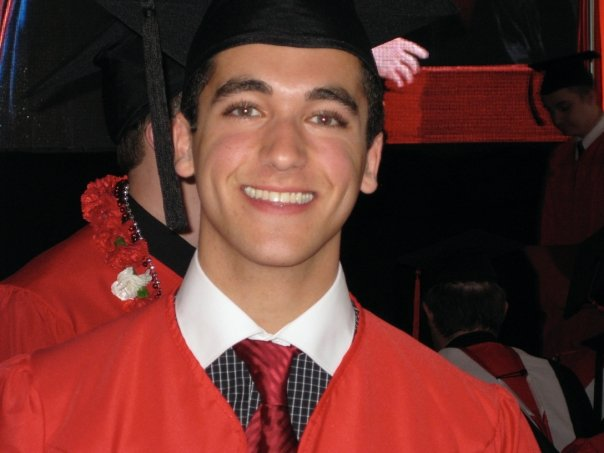
\includegraphics[width=0.23\linewidth]{figs/collegegrad_Soliman} \includegraphics[width=0.15\linewidth]{figs/jobmarket_SolimanA}
\end{figure}		
		\item My first job was teaching math and economics in Dubai

\pause 
		\item I study topics in the economics of crime \& some research questions of interest include
		\begin{enumerate}
			\item What are the impacts of cracking down on rogue doctors during the opioid epidemic on street drug prices, overdose mortality, and other doctors behavior?
			\item Do police respond to changes in punishment severity?
			\item What happens to neighborhood crime when investors buy many properties?
		\end{enumerate}
	\end{wideitemize}
\end{frame}

\begin{frame}{\bf \large A little bit about your classmates (Major and Grad School)}
	
	\begin{figure}[htbp!]
		\centering
		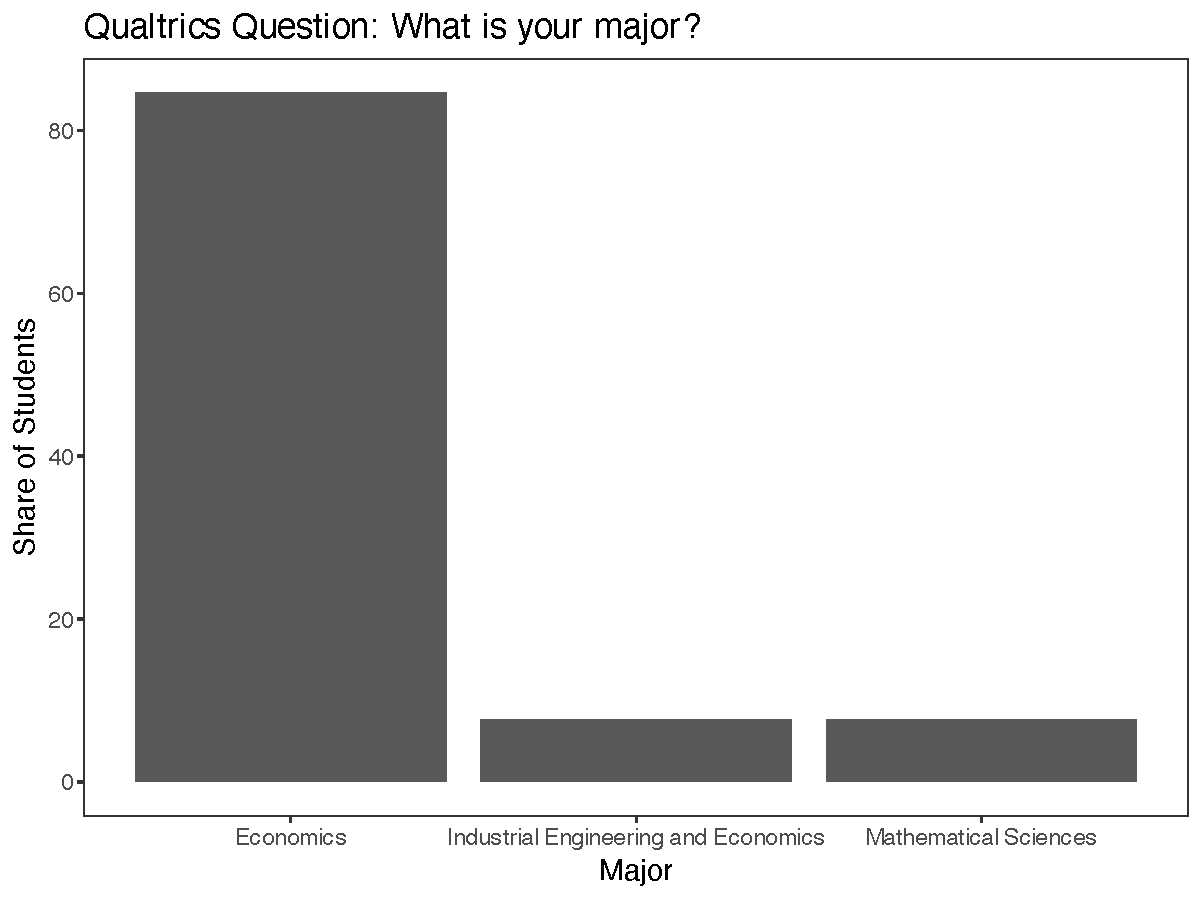
\includegraphics[width=0.54\linewidth]{figs/major_econ4050}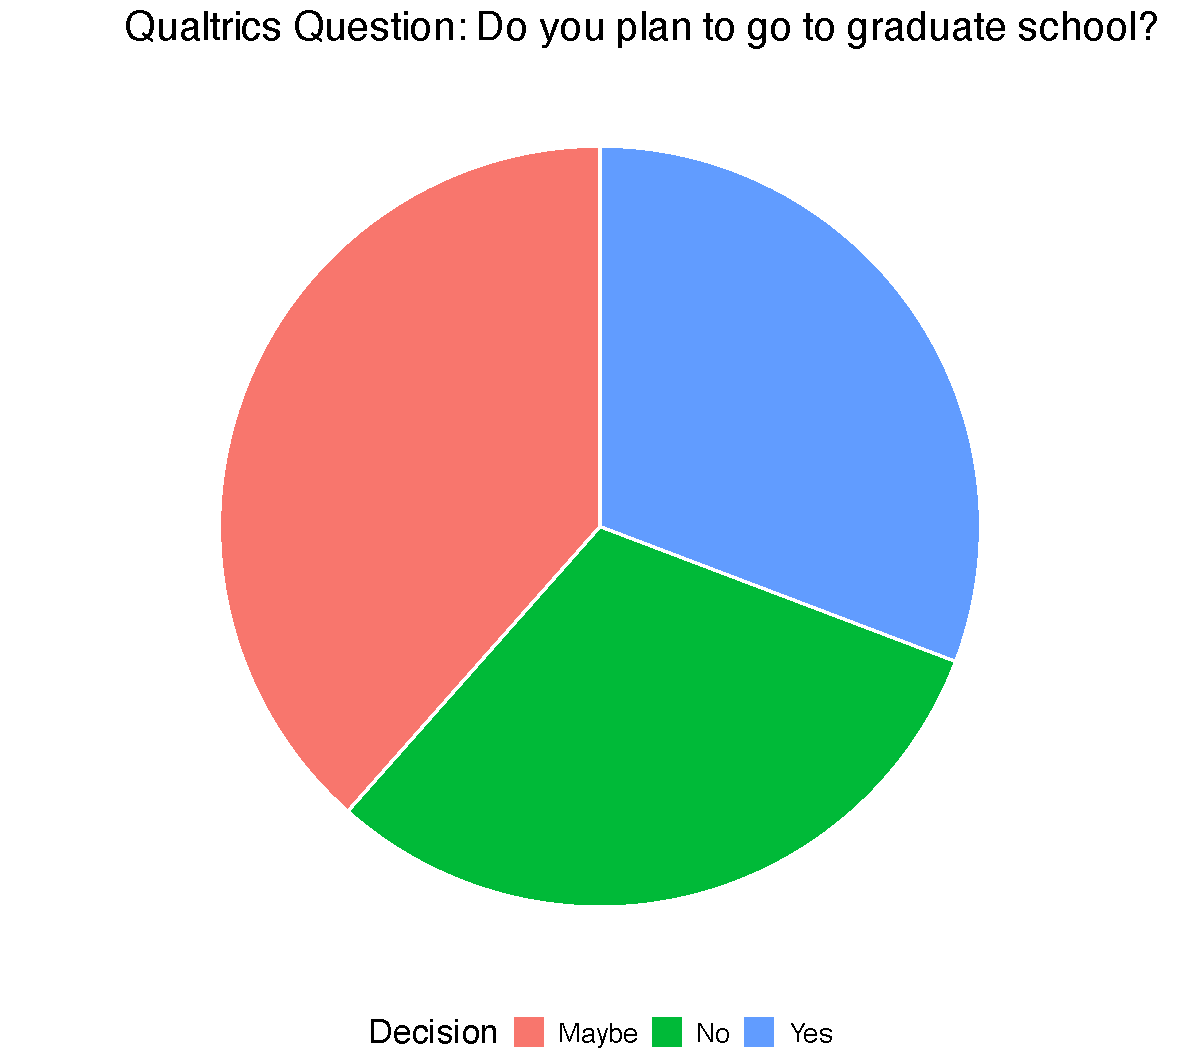
\includegraphics[width=0.46\linewidth]{figs/gradschool_econ4050}
	\end{figure}
\end{frame}

\begin{frame}{\bf \large A little bit about your classmates (Grade and Location)}
	\begin{figure}[htb[!]
		\centering
		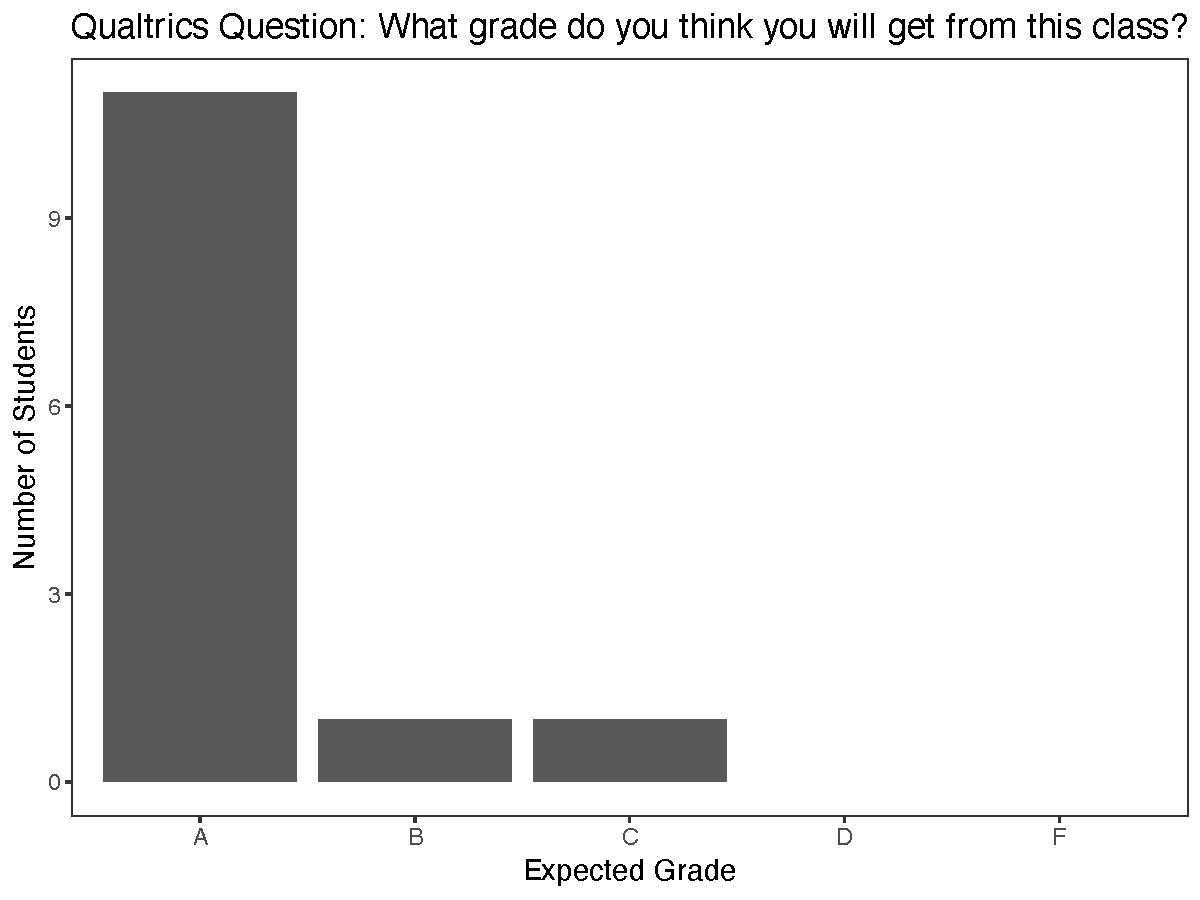
\includegraphics[width=0.46\linewidth]{figs/grade_econ4050}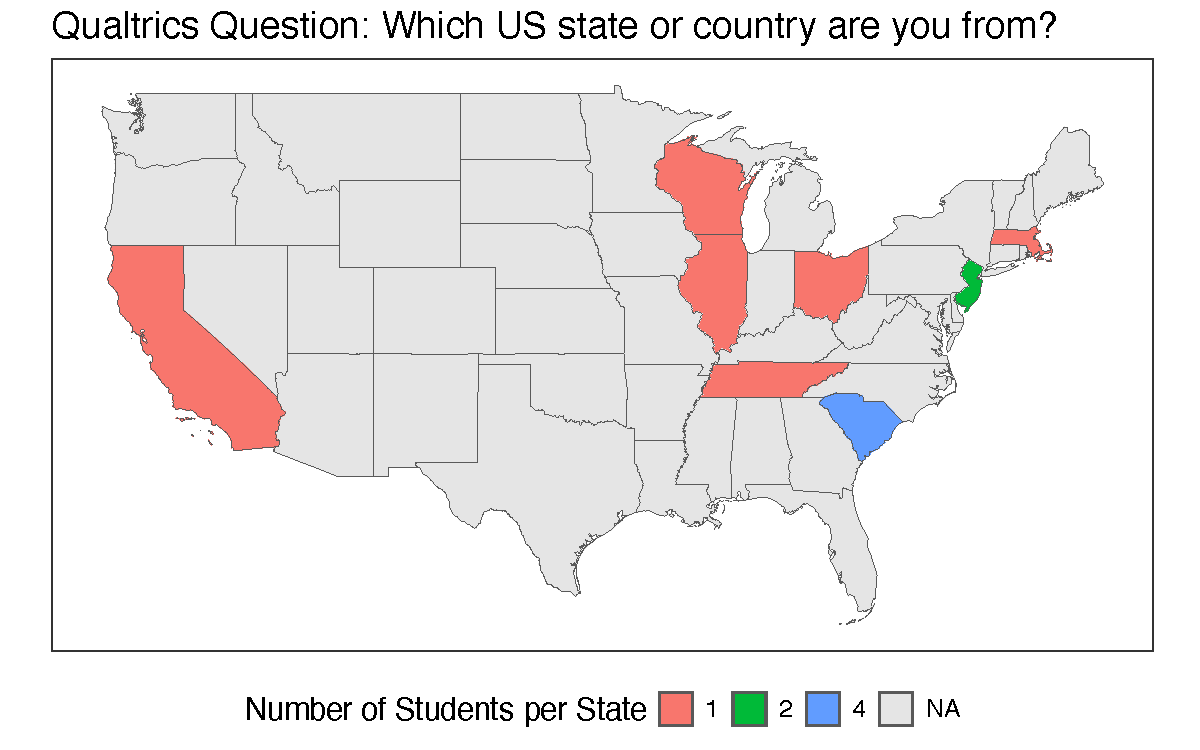
\includegraphics[width=0.54\linewidth]{figs/statemap_econ4050}
	\end{figure}
\end{frame}

\begin{frame}{\bf \large What is econometrics?}
	
	\vspace{0.2cm}
	The statistical toolkit (techniques and methods) that to answer economic \underline{questions} with \underline{data}
	\bigskip 
	
	\pause
	What types of questions might we be interested in: 
	\medskip
	
	\begin{wideitemize}
		\item<1-> Has economic inequality increased since 1960?
		\begin{wideitemize}
			\item<3-> \textbf{Descriptive Question:} asks about how things are (or were) in reality
		\end{wideitemize}
		\item<1-> \href{http://davidcard.berkeley.edu/papers/njmin-aer.pdf}{Does raising the minimum wage reduce employment for low-skilled workers?}
		\begin{wideitemize}
			\item<4-> \textbf{Causal Question:} What would have happened in a counterfactual world?  
		\end{wideitemize}
		\item<1->   What will the unemployment rate be next quarter?
		\begin{wideitemize}
			\item<5-> \textbf{Forecasting Question:} What will happen in the future?  
		\end{wideitemize}

	\end{wideitemize}
	
\end{frame}

\begin{frame}{\bf \large Causal questions will be our focus in this course}
	\begin{wideitemize}
		\item[] More causal questions:
\begin{wideenumerate}
	\item \href{http://davidcard.berkeley.edu/papers/mariel-impact.pdf}{Does immigration \emph{lead to} lower wages and/or higher unemployment for locals? }
	
	\item \href{http://davidcard.berkeley.edu/papers/causal_educ_earnings.pdf}{Does getting a college degree \emph{afford} higher wages? }
	
	\item \href{https://www.imf.org/external/pubs/ft/wp/2014/wp1434.pdf}{Do higher public debt levels \emph{lead to} lower economic growth? }
	\item \href{https://academic.oup.com/qje/article/133/3/1107/4850660}{ Does the
		neighborhood you grew up in have an \emph{impact} on your life outcomes?}
\end{wideenumerate}

\pause 

			\item Note that many other factors could have caused each of these outcomes
			\item Often, we’ll want to focus on the causal impact of just one of these factors (immigration, minimum wage, education, etc.)
			\item Econometrics is about spelling out \textit{conditions} under which we can \textit{claim to measure causal relationships}
			\item We will encounter most basic of those conditions, and talk about some potential pitfalls

	\end{wideitemize}
\end{frame}

\begin{frame}{\bf \large Expectations}
	\begin{wideitemize}
		\item Ask questions: to me, your TA, each other
		\item Make mistakes, but always try
		\item You will be learning a powerful set of skills that apply well outside of this course, so enjoy where you can and try to think of where else they may be useful
	\end{wideitemize}
\end{frame}

\begin{frame}{\bf \large Logistics}
\begin{wideenumerate}
\only<1-1>{
	\vspace{5mm}
	\item[1)] Schedule and Location:
	\begin{wideitemize}
		\item Lectures: 4050-001 TR from 11:00AM to 12:15PM in Powers Hall 207
		\item Lab: 4051-001 T 5:30PM-8:30PM in Powers Hall 112
		\item My office hours are Wednesdays from 3PM to 5PM on Zoom, please sign up in advance for a slot \href{https://shorturl.at/W4luy}{here} 
		\item Our Teaching Assistant (TA) is Haoran Li and will hold office hours (TBD)
	\end{wideitemize}
	
	\item[2)] Content: %and communication:
	
	\begin{wideitemize}
%		\item We will \textbf{exclusively} use Slack for our interactions. Please do not contact me by email unless it is a personal reason
%		\begin{itemize} \item I will be checking Slack sparingly so please help one another in the meantime \end{itemize}
		\item The main course materials are currently posted on \href{https://github.com/adamsoliman/IntroEconometrics}{the Github course website}. Other communication will be via Slack and Canvas.
	\end{wideitemize}}
	
	\pause

	\item[3)] Software:

\begin{wideitemize}
	\item R for statistical analyses (to be covered in Lab sessions and throughout the course)
\end{wideitemize}

\item[4)] Assessments:
\begin{wideitemize}
	\item In-class quizzes/attendance: 10\%
	\item Lab work: 25\%
	\item 1 midterm exam: 25\%
	\item Final project and associated presentation: 30\% and 10\%, respectively
\end{wideitemize}

	\item[5)] Prerequisites:
\begin{wideitemize}
	\item ECON2110 and 2120 Principle of Microeconomics and Macroeconomics 
	\item MATH1080 Calculus One
	\item STAT3090/MATH3090 Introduction to Statistics
\end{wideitemize}
\end{wideenumerate}
\end{frame}

\begin{frame}{\bf \large Resources}
\begin{wideitemize}
	\item \textbf{Econometrics}
\begin{wideitemize}
	\item \href{https://scpoecon.github.io/ScPoEconometrics/index.html}{SciencesPo Online Book}
	\item \href{https://mixtape.scunning.com/}{Causal Inference: The Mixtape by Cunningham}
	\item \href{https://www.youtube.com/user/SpartacanUsuals}{Ben Lambert's youtube channel}
\end{wideitemize}
			\item \textbf{Metrics and `R'}
\begin{wideitemize}
	\item \href{https://moderndive.com/}{ModernDive}
	\item \href{https://www.econometrics-with-r.org/}{Introduction to Econometrics with R}
	\item \href{https://github.com/iamericfletcher/awesome-r-learning-resources}{Awesome R Learning Resources}
	\item \href{https://r4ds.hadley.nz/}{R for Data Science}
\end{wideitemize}	
\end{wideitemize}
	
\end{frame}

\section{Why is Econometrics Challenging?}
	\begin{frame}[plain, noframenumbering]{\bf \large Outline}
	\tableofcontents[currentsection]
\end{frame}
\begin{frame}{\bf \large Why is answering these questions hard?}

\begin{wideitemize}
\item
For descriptive questions: we only observe data for a \textbf{sample} of individuals, not for the full \textbf{population}
	\begin{wideitemize}
		\item 
		Example: we want to know how the distribution of income in the US has changed, but we only observe income for a survey of workers
	\end{wideitemize}
\pause

\item Best case scenario: Our sample is \textbf{randomly} selected from the population \\
	\begin{wideitemize}
		\item 
		For example, workers in the survey were drawn out of hat with names of all possible workers

	\end{wideitemize}

\pause 

\item Worst case scenario: Our sample is \textit{not representative} of the population that we care about
	\begin{wideitemize}
		\item For example, workers with certain characteristics were more likely to respond to the survey
	\end{wideitemize}
\end{wideitemize}

\end{frame}


\begin{frame}{\bf \large An example from before we were born \only<2-2>{$\implies$ error known as \textit{selection bias}}}
\centering
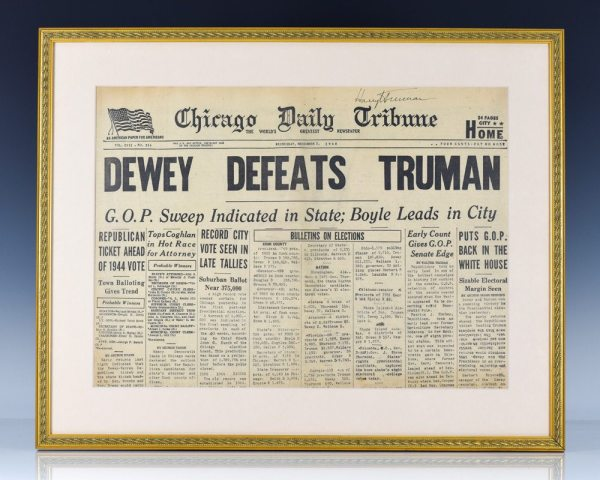
\includegraphics[width = 0.4\linewidth]{figs/dewey-defeats-truman}
\begin{wideitemize}
	\item 
	In 1948, Chicago Tribune writes that Thomas Dewey defeats Harry Truman in the 1948 presidential election, based on survey of voters.
	
	\pause
	\item
	But their survey was conducted by phone. In 1948, only rich people had phones: sample $\neq$ population $\implies$ misleading results! 
\end{wideitemize}
\end{frame}


\begin{frame}{\bf \large Why is answering these questions hard? (Part II)}
\begin{wideitemize}
	\item
	Answering causal questions is often \textit{even harder} than descriptive ones because they involve \underline{both} a descriptive component (what are outcomes in reality?) and a \textit{counterfactual} component (how would things have been under a different treatment?)
	
	\pause
	\item
	Example: what is the causal effect on your earnings of going to Clemson instead of USC? 
		\begin{wideitemize}
			\item
			Descriptive Question: how much do Clemson students earn after graduation? 
			
			\item
			Counterfactual Question: how much would Clemson students have earned if they went to USC?  
		\end{wideitemize}
		

	\item Counterfactual questions can't ever be answered with data alone. Need additional assumptions to learn about them!	
\end{wideitemize}	
\end{frame}



\begin{frame}{\bf \large Splitting up the problem}
	\begin{wideitemize}
		
		\item
		When thinking about causal questions, it's often easier to split the problem in two
		
		\item
		\textbf{Identification:} what could we learn about the parameters we care about (causal effects) if we had the \text{observable data} for the entire population
		\begin{wideitemize}
			\item 
			Need to make assumptions about how observed outcomes relate to outcomes that would have been realized under different treatments
		\end{wideitemize}
		
		\item
		\textbf{Statistics}: what can we learn about the full population that we care about from the finite sample that we have?
			\begin{wideitemize}
				\item 
				Need to understand the process by which our data is generated from the full population
			\end{wideitemize} 	
		
	\end{wideitemize}	
	
\end{frame}



\begin{frame}{\bf \large Framework for thinking about these steps}
	
\begin{wideitemize}

\item \textbf{Sample:} the data that you actually observe
	\begin{wideitemize}
		\item
		A survey of students from Clemson and USC graduates about their earnings 
	\end{wideitemize}

\item \textbf{Estimator:} a function of the data in the sample 
	\begin{wideitemize}
		\item Difference in earnings between Clemson and USC students in survey
	\end{wideitemize}

\item \textbf{Estimand:} a function of the observable data for the \textit{population}
	\begin{wideitemize}
		\item Difference in earnings between all Clemson and USC students 
	\end{wideitemize}

\item \textbf{Target (aka structural) parameter:} what we actually care about
	\begin{wideitemize}
		\item Causal effect on earnings of going to Clemson relative to USC
	\end{wideitemize}

\end{wideitemize}	

\medskip
\pause
\begin{wideitemize}

\item The process of learning about the \textit{estimand} from the \text{estimator} constructed with your \textit{sample} is called \textbf{statistical estimation/inference}

\item The process of learning about the \textit{parameter} from the \textit{estimand} is called \textbf{identification}

\end{wideitemize}	
\end{frame}

\begin{comment}
	\begin{frame}
		\begin{figure}
			\centering
			\includegraphics[width=\textwidth]{figs/BigPicture}
		\end{figure}
	\end{frame}
\end{comment}


\begin{frame}{\bf \large Let's add some math...by introducing \textbf{potential outcomes} notation}
\begin{wideitemize}
	
	\item $D_i$ = indicator if get treatment (1 if Clemson, 0 if USC)
	

	\item $Y_i(1)$ = outcome under treatment = earnings at Clemson
	\item $Y_i(0)$ = outcome under control = earnings at USC
	
\vspace{10mm}

	\item Observed outcome $Y_i$ is $Y_i(1)$ if $D_i = 1$ and $Y_i(0)$ if $D_i = 0$. ($Y_i$ is your actual earnings)
	
	\item
	We can write the observed outcome as $Y_i = D_i Y_i(1) + (1-D_i) Y_i(0)$
\end{wideitemize}

\end{frame}



\begin{frame}{\bf \large What is the causal effect on earnings of going to Clemson instead of USC?}
\begin{wideitemize}
	\item
	\textbf{Sample}: $(Y_i,D_i)$ for $i=1,...N$. Data with earnings and where you went to school
	
	\pause 
	
	\item
	\textbf{Estimator}: Difference in sample mean of earnings for people who went to Clemson and people who went to USC: 
			
			$$ \underbrace{\frac{1}{N_1} \sum_{i:D_i=1} Y_i}_{\text{Avg earnings at Clemson in sample}} - \underbrace{\frac{1}{N_0} \sum_{i:D_i=0} Y_i}_{\text{Avg earnings at USC in sample}}$$		

	
	\pause
		\item
		\textbf{Estimand}: 
			Difference in population mean of earnings for people went to Clemson and people who went to USC: 
			
			$$\underbrace{ E[ Y_i | D_i = 1] }_{\text{Avg earnings at Clemson in population}} - \underbrace{E[Y_i | D_i = 0]}_{\text{Avg earnings at USC in population}}$$
		 
	\pause 
	
	\item \textbf{Target parameter}: Causal effect of Clemson for Clemson students:
			$\underbrace{E[Y_i(1) | D_i =1]}_{\text{Earnings at Clemson for Clemson students in pop}} - \underbrace{E[Y_i(0) | D_i = 1]}_{\text{Earnings at USC for Clemson students in pop}} $ 
		\end{wideitemize}
\end{frame}


\begin{frame}{\bf \large Why is causal identification hard?}
	
	\begin{wideitemize}
		
		\item
		Thought experiment: suppose we had data on earnings for \textit{every} Clemson and USC graduate
		
		
		\item
		We can learn from the data:
		$$\color{teal} \underbrace{E[ Y_i(1) | D_i=1  ] }_{\text{Earnings at Clemson for Clemson Students}} \hspace{0.5cm}  \text{and} \hspace{0.5cm} \underbrace{E[Y_i(0) | D_i = 0]	}_{\text{Earnings at USC for USC students}}$$
		
		\pause 
		\item
		The causal effect of Clemson for Clemson students is 
		$$ \color{teal}{\underbrace{E[ Y_i(1) | D_i=1  ] }_{\text{Earnings at Clemson for Clemson Students}}} - \color{red}{ \underbrace{E[ Y_i(0) | D_i=1  ] }_{\text{Earnings at USC for Clemson Students}}}$$ 
		
		\pause 
		\item
		The data doesn't tell us $\color{red}{ \underbrace{E[ Y_i(0) | D_i=1 ] }_{\text{Earnings at USC for Clemson Students}}}$. Why not? 
%\pause			\begin{wideitemize} \item Because we never see Clemson students going to USC! \end{wideitemize} 
		
	\end{wideitemize}
	
\end{frame}


\begin{frame}
	\begin{wideitemize}
		\item
		One idea to solve this problem would be to assume that: 
		
		$$ \color{red}{ \underbrace{E[ Y_i(0) | D_i=1  ] }_{\text{Earnings at USC for Clemson Students}}} = \color{teal}{ \underbrace{E[ Y_i(0) | D_i=0 ] }_{\text{Earnings at USC for USC Students}}}$$
		
		\item
		Why might this give us the wrong answer? 
		
		\pause
		
		\item
		Because Clemson students may be different from USC students in other ways that would affect their earnings (regardless of where they went to college)
		
			\begin{wideitemize}
				\item 
				Academic ability, family background, career goals, etc.
			\end{wideitemize}
		
		\item
		These differences are referred to as \textit{omitted variables} or \textit{confounding factors}
	\end{wideitemize}
\end{frame}

\begin{frame}{\bf \large What about experiments?}
\begin{wideitemize}
\item
The gold standard for learning about causal effects is a randomized controlled trial (RCT), aka experiment

\item
Suppose that the Clemson and USC administration randomized who got into which college (assume these are the only 2 colleges for simplicity)

\item
Since college is randomly assigned, the only thing that differs between Clemson and USC students is the college they went to

\item
Hence, 

		$$ \color{red}{ \underbrace{E[ Y_i(0) | D_i=1  ] }_{\text{Earnings at USC for Clemson Students}}} = \color{teal}{ \underbrace{E[ Y_i(0) | D_i=0 ] }_{\text{Earnings at USC for USC Students}}}$$
		
		since we've eliminated any confounding factors


\end{wideitemize}
\end{frame}

\begin{frame}{\bf \large But running experiments is often hard/impossible}
	\begin{wideitemize}
	
	\item
	Unfortunately, Clemson/USC have not let us randomize who gets into which college
		\begin{wideitemize}
			\item
			At least not yet! If you could convince them to do this, it'd make for a cool senior thesis! 
		\end{wideitemize}


	\item
	Likewise, it is difficult to convince states to randomize their minimum wages, or other policies
	
	\item
	In some cases, randomization is not just difficult but would be immoral 
	
		\begin{wideitemize}
			\item 
			``What is the causal effect of spousal death on labor supply?''
		\end{wideitemize}	
	
	\item
	In this course, we'll discuss tools economists try to use when running experiments is not possible
	\end{wideitemize}
\end{frame}

\section{Course Roadmap}
	\begin{frame}[plain, noframenumbering]{\bf \large Outline}
	\tableofcontents[currentsection]
\end{frame}
\begin{frame}{\bf \large Course Roadmap -- Where we're going}

\begin{minipage}{.5\textwidth}
\begin{wideitemize}
	\item \textbf{Topics}
	\begin{wideenumerate}
		\item Simple Linear Regression 
		\item Introduction to Causality
		\item Multiple Linear Regression
		\item Linear Regression Extensions
		\item Sampling
		\item Confidence Intervals \& Hypothesis Testing
		\item Regression Inference
		\item Regression Discontinuity
		\item Instrumental Variables
		\item Difference-in-Differences
		\item Panel Data
	\end{wideenumerate}
\end{wideitemize}
\end{minipage}\pause%
\begin{minipage}{.5\textwidth}
	\begin{wideitemize}
		\item \textbf{Important Dates}
		\begin{wideitemize}
			\item	October 3rd: No Class
			\item	October 15th: No Class (Fall Break)
			\item	October 16th-17th: Midterm Exam (Take home, No Lecture)
			\item	November 5th: No Class (Election Day)
			\item	November 28th: No Class (Thanksgiving Break)
			\item	Final Project Presentations: November 21st, November 26th, December 3rd, and December 5th 
		\end{wideitemize}
	\end{wideitemize}
\end{minipage}
\end{frame}

\begin{comment}
	\begin{frame}{\bf \large And now...}
		\LARGE	A brief introduction to R
	\end{frame}
\end{comment}

\end{document}

